\documentclass{article}

\usepackage{graphicx}
\usepackage{tikz}
\usepackage{tikzsymbols}
\usetikzlibrary{calc,patterns,shapes.geometric}
\pagestyle{empty}
\usepackage[margin=0pt]{geometry}
\geometry{papersize={14in,12in}}

\def\centerarc[#1](#2)(#3:#4:#5){\draw[#1] ($(#2)+({#5*cos(#3)},{#5*sin(#3)})$) arc (#3:#4:#5);}

\begin{document}
	\begin{figure}
		\centering
		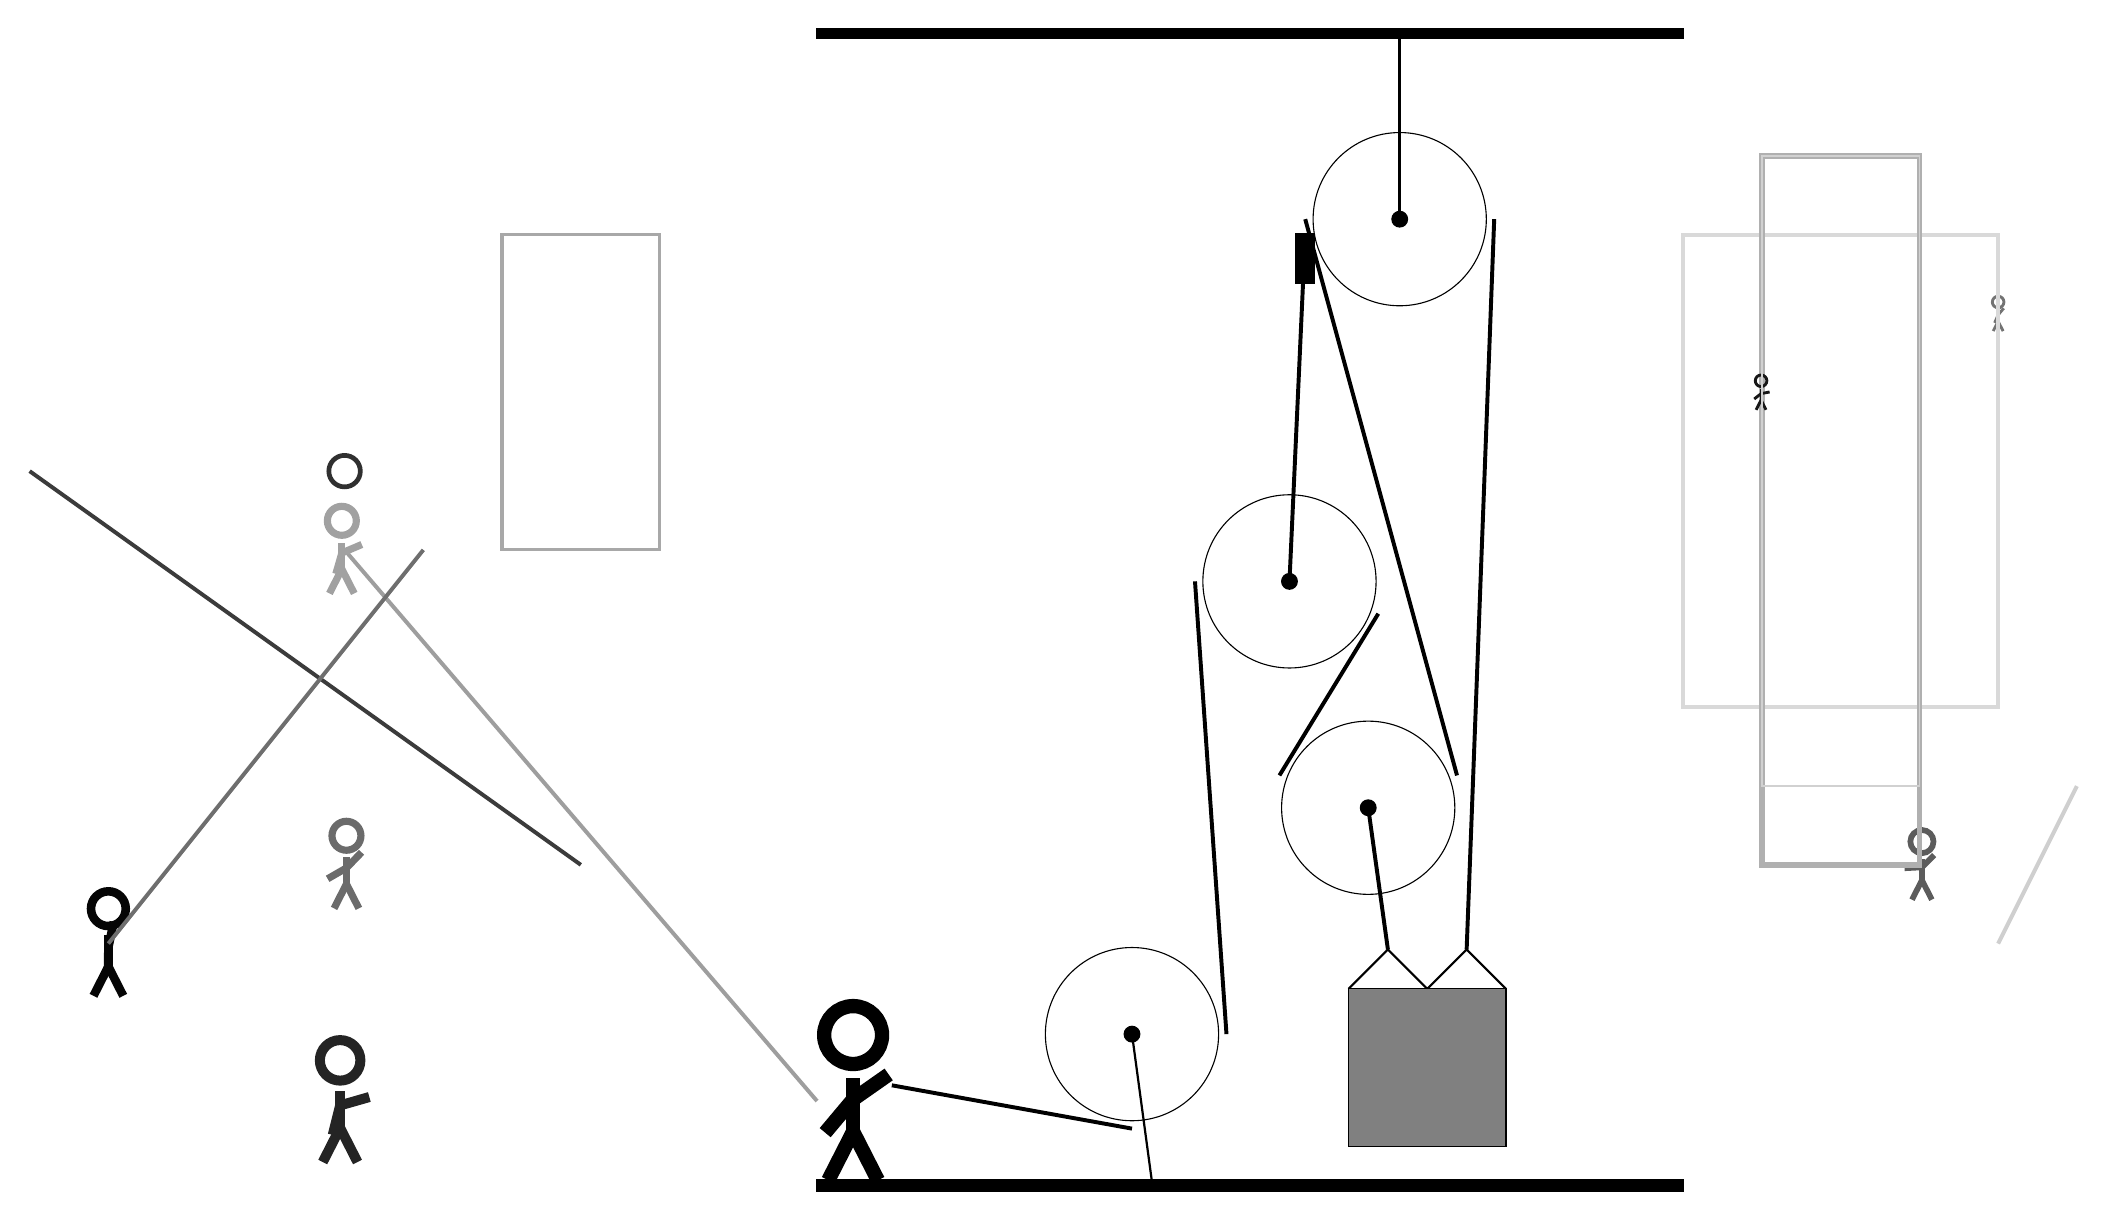
\begin{tikzpicture}
			%%%%% START %%%%%
			
			\draw[fill=black] (-6, 11.5) rectangle (5, 11.625);
			
			\draw (0, 4.6) circle (1.1);
			\draw[fill=black] (0, 4.6) circle (0.1);
			
			\draw (1, 1.725) circle (1.1);
			\draw[fill=black] (1, 1.725) circle (0.1);
			
			\draw[line width=0.5mm, color=black!77](-9, 1) -- (-16, 6);
			
			\node[line width=0.7mm, color=black!98] at (-15, 0) {\Strichmaxerl[6][89][78]};
			\draw[line width=0.5mm, color=black!38](-6, -2) -- (-12, 5);
			\node[line width=0.6mm, color=black!58] at (-12, 1) {\Strichmaxerl[5][30][46]};
			\draw [line width=0.6mm, color=black!81](-12, 6) circle (0.2);
			\draw[line width=0.5mm, color=black!57](-11, 5) -- (-15, 0);
			\draw[line width=0.4mm, color=black!34] (-8, 5) rectangle (-10, 9);
			
			\node[line width=0.3mm, color=black!64] at (8, 1) {\Strichmaxerl[4][3][45]};
			\node[line width=0.4mm, color=black!37] at (-12, 5) {\Strichmaxerl[5][74][23]};
			\node[line width=0.6mm, color=black!55] at (9, 8) {\Strichmaxerl[2][66][50]};
			\draw[line width=0.5mm, color=black!15] (5, 3) rectangle (9, 9);
			\draw[line width=0.7mm, color=black!31] (6, 10) rectangle (8, 1);
			\node[line width=0.5mm, color=black!91] at (6, 7) {\Strichmaxerl[2][38][11]};
			
			\draw[line width=0.5mm, color=black!19](10, 2) -- (9, 0);
			\draw[line width=0.2mm, color=black!18] (6, 10) rectangle (8, 2);
			\node[line width=0.7mm, color=black!86] at (-12, -2) {\Strichmaxerl[7][76][16]};
			
			
			\draw (1.4, 9.2) circle (1.1);
			\draw[fill=black] (1.4, 9.2) circle (0.1);
			\draw[very thick] (1.4, 9.2) -- (1.4, 11.5);
			
			\draw (-2, -1.15) circle (1.1);
			\draw[fill=black] (-2, -1.15) circle (0.1);
			\draw[thick] (-2, -1.15) -- (-1.75, -3);
			
			
			\draw[thick]  (0.75, -0.575) -- (1.25, -0.075) -- (1.75, -0.575) -- (2.25, -0.075) -- (2.75, -0.575);
			\draw[fill=black!50] (0.75, -0.575) rectangle (2.75, -2.575);
			\draw[line width=0.5mm] (-5.05, -1.8) -- (-2, -2.35);
			\centerarc[line width=0.5mm](-2, -1.15)(270:360:1.2000000000000002);
			\draw[line width=0.5mm] (-0.8, -1.15) -- (-1.2, 4.6);
			\draw[line width=0.5mm] (0, 4.6) -- (0.2, 9.0);
			\draw[line width=0.5mm, fill=black](0.1, 8.4) rectangle (0.3, 9.0);
			\centerarc[line width=0.5mm](0, 4.6)(-20:180:1.2000000000000002);
			\draw[line width=0.5mm] (1.1276, 4.1896) -- (-0.1276, 2.1354);
			\centerarc[line width=0.5mm](1, 1.725)(160:380:1.2000000000000002);
			\draw[line width=0.5mm] (2.1276, 2.1354) -- (0.2, 9.2);
			\draw[line width=0.5mm](1, 1.725) -- (1.25, -0.075);
			\centerarc[line width=0.5mm](1.4, 9.2)(0:180:1.2000000000000002);
			\draw[line width=0.5mm] (2.6, 9.2) -- (2.25, -0.075);
			
			\node at (-5.5, -1.9) {\Strichmaxerl[10][50][35]};
			
			\draw[fill=black] (-6, -3) rectangle (5, -3.15);
			
			%%%%% END %%%%%
		\end{tikzpicture}
	\end{figure}	
\end{document}